%Version 3.1 December 2024
% See section 11 of the User Manual for version history
%
%%%%%%%%%%%%%%%%%%%%%%%%%%%%%%%%%%%%%%%%%%%%%%%%%%%%%%%%%%%%%%%%%%%%%%
%%                                                                 %%
%% Please do not use \input{...} to include other tex files.       %%
%% Submit your LaTeX manuscript as one .tex document.              %%
%%                                                                 %%
%% All additional figures and files should be attached             %%
%% separately and not embedded in the \TeX\ document itself.       %%
%%                                                                 %%
%%%%%%%%%%%%%%%%%%%%%%%%%%%%%%%%%%%%%%%%%%%%%%%%%%%%%%%%%%%%%%%%%%%%%

%%\documentclass[referee,sn-basic]{sn-jnl}% referee option is meant for double line spacing

%%=======================================================%%
%% to print line numbers in the margin use lineno option %%
%%=======================================================%%

%%\documentclass[lineno,pdflatex,sn-basic]{sn-jnl}% Basic Springer Nature Reference Style/Chemistry Reference Style

%%=========================================================================================%%
%% the documentclass is set to pdflatex as default. You can delete it if not appropriate.  %%
%%=========================================================================================%%

%%\documentclass[sn-basic]{sn-jnl}% Basic Springer Nature Reference Style/Chemistry Reference Style

%%Note: the following reference styles support Namedate and Numbered referencing. By default the style follows the most common style. To switch between the options you can add or remove “Numbered” in the optional parenthesis. 
%%The option is available for: sn-basic.bst, sn-chicago.bst%  
 
%%\documentclass[pdflatex,sn-nature]{sn-jnl}% Style for submissions to Nature Portfolio journals
%%\documentclass[pdflatex,sn-basic]{sn-jnl}% Basic Springer Nature Reference Style/Chemistry Reference Style
\documentclass[pdflatex,sn-mathphys-num]{sn-jnl}% Math and Physical Sciences Numbered Reference Style
%%\documentclass[pdflatex,sn-mathphys-ay]{sn-jnl}% Math and Physical Sciences Author Year Reference Style
%%\documentclass[pdflatex,sn-aps]{sn-jnl}% American Physical Society (APS) Reference Style
%%\documentclass[pdflatex,sn-vancouver-num]{sn-jnl}% Vancouver Numbered Reference Style
%%\documentclass[pdflatex,sn-vancouver-ay]{sn-jnl}% Vancouver Author Year Reference Style
%%\documentclass[pdflatex,sn-apa]{sn-jnl}% APA Reference Style
%%\documentclass[pdflatex,sn-chicago]{sn-jnl}% Chicago-based Humanities Reference Style

%%%% Standard Packages
%%<additional latex packages if required can be included here>

\usepackage{graphicx}%
\usepackage{multirow}%
\usepackage{amsmath,amssymb,amsfonts}%
\usepackage{amsthm}%
\usepackage{mathrsfs}%
\usepackage[title]{appendix}%
\usepackage{xcolor}%
\usepackage{textcomp}%
\usepackage{manyfoot}%
\usepackage{booktabs}%
\usepackage{algorithm}%
\usepackage{algorithmicx}%
\usepackage{algpseudocode}%
\usepackage{listings}%
\usepackage{placeins}
\usepackage{float}
\usepackage{array}
\newcolumntype{L}[1]{>{\raggedright\arraybackslash}p{#1}}

%%%%

%%%%%=============================================================================%%%%
%%%%  Remarks: This template is provided to aid authors with the preparation
%%%%  of original research articles intended for submission to journals published 
%%%%  by Springer Nature. The guidance has been prepared in partnership with 
%%%%  production teams to conform to Springer Nature technical requirements. 
%%%%  Editorial and presentation requirements differ among journal portfolios and 
%%%%  research disciplines. You may find sections in this template are irrelevant 
%%%%  to your work and are empowered to omit any such section if allowed by the 
%%%%  journal you intend to submit to. The submission guidelines and policies 
%%%%  of the journal take precedence. A detailed User Manual is available in the 
%%%%  template package for technical guidance.
%%%%%=============================================================================%%%%

%% as per the requirement new theorem styles can be included as shown below
\theoremstyle{thmstyleone}%
\newtheorem{theorem}{Theorem}%  meant for continuous numbers
%%\newtheorem{theorem}{Theorem}[section]% meant for sectionwise numbers
%% optional argument [theorem] produces theorem numbering sequence instead of independent numbers for Proposition
\newtheorem{proposition}[theorem]{Proposition}% 
%%\newtheorem{proposition}{Proposition}% to get separate numbers for theorem and proposition etc.

\theoremstyle{thmstyletwo}%
\newtheorem{example}{Example}%
\newtheorem{remark}{Remark}%

\theoremstyle{thmstylethree}%
\newtheorem{definition}{Definition}%

\raggedbottom
%%\unnumbered% uncomment this for unnumbered level heads

\renewcommand{\topfraction}{0.9}
\renewcommand{\bottomfraction}{0.8}
\renewcommand{\textfraction}{0.07}
\renewcommand{\floatpagefraction}{0.85}
\setcounter{topnumber}{3}
\setcounter{totalnumber}{5}
\begin{document}

\title[EEG Motor Action and Motor Imagery Classification]{EEG-Based Motor Action and Motor Imagery Classification Using Machine Learning}

\author[1]{\fnm{Harsada} \sur{K}}\email{cb.ai.u4aid24019@cb.students.amrita.edu}
\author[1]{\fnm{V} \sur{Tanay Darshan}}\email{cb.ai.u4aid24059@cb.students.amrita.edu}
\author[1]{\fnm{K} \sur{Nikhitha}}\email{cb.ai.u4aid24042@cb.students.amrita.edu}
\author[1]{\fnm{S Sai} \sur{Tejesh Reddy}}\email{cb.ai.u4aid24057@cb.students.amrita.edu}
\author*[1]{\fnm{Abhishek} \sur{S}}\email{s\_abhishek@cb.amrita.edu}

\affil*[1]{\orgdiv{Amrita School of Artificial Intelligence, Coimbatore}\\ \orgname{Amrita Vishwa Vidyapeetham}, \country{India}}

\abstract{This work presents an EEG-based classification framework for distinguishing motor actions and motor imagery using a consumer-grade Emotiv EPOC X headset. EEG was recorded from 47 participants (14 channels, 128 Hz) while they performed or imagined six limb movements of the right and left arms, legs and wrists, giving twelve task classes. The start of each task schedule was estimated from the headset's motion sensor, since it varied between recordings. Signals were band-pass filtered (4--45 Hz), cleaned by amplitude- and kurtosis-based trial rejection, and split into 2-second windows, yielding 8,092 windows from 476 trials. Each window was described by spectral, statistical, fractal and wavelet features, along with spectrogram, scalogram, connectivity and Riemannian tangent-space features, standardised per recording. An ensemble of Logistic Regression, Linear Discriminant Analysis, Extra Trees and Histogram Gradient Boosting, trained with hemispheric mirror augmentation, classified the windows, and predictions were averaged within each trial. SVM, Random Forest, Naive Bayes, AdaBoost, EEGNet and CNN--LSTM models were evaluated for comparison. Using person-wise GroupKFold validation, the ensemble achieved 80.25\% for action-versus-imagery, 26.68\% for body-part, 21.43\% for twelve-class, and 58.09\% for left-versus-right imagery classification.}

\keywords{Electroencephalography (EEG), Brain--Computer Interface, Motor Imagery, Motor Action, Spectrogram, Scalogram, Riemannian Geometry, Machine Learning, Emotiv EPOC X}

\maketitle

%% ===================================================================
\section{Introduction}\label{sec1}

Brain--computer interfaces (BCIs) translate brain activity into commands a computer can use, which matters most for motor applications, where the intention to move remains visible in cortical activity even when movement is limited. EEG is the usual choice because it is non-invasive, fast and portable \citep{Wolpaw2002}.

Motor execution and motor imagery are closely related but not the same. In execution the participant actually moves; in imagery the movement is only rehearsed in the mind. Both change the sensorimotor rhythms, mainly in the mu (8--12 Hz) and beta (13--30 Hz) bands, and these changes are the basis of most motor BCIs \citep{Pfurtscheller2001}. Early systems mostly separated left- from right-hand imagery with Common Spatial Patterns (CSP) and a linear classifier \citep{Ramoser2000,Blankertz2008}. The problem becomes much harder once several body parts are involved, because their cortical areas lie close together, scalp EEG blurs them, and the signal varies a lot from person to person \citep{Lotte2018}.

Hardware adds another constraint. Clinical amplifiers give clean signals but are costly and slow to set up, while consumer headsets such as the Emotiv EPOC family are cheap and quick to wear but noisier and with fewer, differently placed electrodes \citep{Badcock2013}.

This study builds a complete pipeline around a 14-channel Emotiv EPOC X and a twelve-task protocol: six movements (right and left arm, leg and wrist), each performed and then imagined. The same recordings are analysed at several levels of difficulty, and every result is subject-independent: the model is always tested on people whose data it never saw. The main contributions are:

\begin{enumerate}
\item \textbf{A twelve-task motor dataset from consumer-grade EEG,} recorded from 47 participants with a 14-channel Emotiv EPOC X while they performed and imagined six limb movements.
\item \textbf{Multi-level motor classification.} The recordings are analysed as action versus imagery (2 classes), body part (6 classes) and exact task (12 classes), showing how performance changes as the target becomes more specific.
\item \textbf{Time--frequency and multi-domain feature fusion.} Handcrafted spectral, statistical, fractal and wavelet features are combined with spectrogram (STFT), scalogram (CWT), connectivity and Riemannian features, and the value of each family is measured separately.
\item \textbf{Cross-subject adaptation and trial-level decisions.} Features are standardised per recording without labels, training data are doubled by hemispheric mirror augmentation, and an ensemble of four classifiers makes one decision per trial.
\end{enumerate}

%% ===================================================================
\section{Literature Review}\label{sec:related}

\subsection{Sensorimotor rhythms, execution and imagery}
Moving a limb, or only imagining it, lowers the power of the mu and beta rhythms over the opposite motor cortex; the power recovers, often with a short rebound, once the movement ends. These event-related desynchronisation and synchronisation (ERD/ERS) patterns were described decades ago and remain the physiological basis of motor decoding \citep{PfurtschellerLopes1999,Pfurtscheller2001}. Imagery produces the same kind of ERD as execution, but weaker and less focused, which is why separating the two is possible but not trivial. Wang et al.\ classified hand execution against imagery in 30 participants: a simple beta-rebound rule reached 59.77\%, and an SVM on statistical, wavelet, power, entropy and CSP features reached 79.51\% \citep{Wang2022}. On the 109-subject PhysioNet data, Shuqfa et al.\ decoded four-class execution and imagery with Riemannian classifiers and obtained up to 81.5\% for execution and 76.4\% for imagery, showing that executed movements are consistently easier to decode than imagined ones \citep{Shuqfa2023}.

\subsection{Spatial filtering and Riemannian geometry}
Common Spatial Patterns finds channel combinations whose variance differs most between two classes. Ramoser et al.\ introduced it for left/right hand imagery, with accuracies of roughly 80--90\% in their three subjects \citep{Ramoser2000}, and later work made it more robust to noise and small training sets through regularisation \citep{Blankertz2008}. Filter-bank CSP (FBCSP) applies CSP in several frequency sub-bands and selects the most useful ones; it won the BCI Competition IV and reached about 68\% on its four-class data set \citep{Ang2012}. Covariance-based methods go one step further: each trial is represented by its channel covariance matrix and classified with Riemannian geometry, either by distance to class means or after mapping to a tangent space \citep{Barachant2012}. For multi-class tasks with complex movements, Lee et al.\ found that simple time-domain features with shrinkage LDA can outperform CSP and spectral features \citep{LeeSB2019}, a reminder that the best representation depends on the task.

\subsection{Time--frequency representations}
Because ERD is a change over time, several studies keep the time axis rather than averaging power over a window. Tabar and Halici turned short-time Fourier transform (STFT) spectrograms into images and classified them with a CNN and stacked autoencoder, reaching about 77\% on two-class BCI Competition IV-2b data \citep{Tabar2017}. Wavelets offer a better time--frequency trade-off, using short windows for fast rhythms and long ones for slow rhythms \citep{Torrence1998}. Xu et al.\ combined wavelet time--frequency images of C3, Cz and C4 and reached 90\% on BCI Competition II data with a small CNN \citep{Xu2019}, and Lee and Choi built scalogram images from the continuous wavelet transform (CWT) with three mother wavelets and improved on earlier results on two public data sets \citep{LeeChoi2019}. These studies used research-grade EEG with central electrodes and subject-specific training; how spectrograms and scalograms compare on a consumer headset in a cross-subject setting has received little attention.

\subsection{Deep learning}
Convolutional networks can learn spatial and temporal filters directly from raw EEG. Schirrmeister et al.\ showed that deep and shallow ConvNets match FBCSP on four-class imagery (about 71--74\%) \citep{Schirrmeister2017}, and EEGNet reached competitive performance across several BCI paradigms with only a few thousand parameters \citep{Lawhern2018}. Reviews note, however, that the advantage of deep models shrinks when training data are limited or when recording conditions differ from benchmark sets \citep{Roy2019}.

\subsection{Cross-subject generalisation}
A model trained on some people usually loses accuracy on new ones, because anatomy, electrode contact and imagery strategy shift the EEG distribution. Alignment methods reduce this by re-centring each person's data before classification, in Euclidean space \citep{He2020} or on the Riemannian manifold \citep{Zanini2018}. These methods need only unlabelled data from the new person, which makes them practical for BCIs.

\subsection{Consumer-grade EEG for motor imagery}
The Emotiv EPOC was designed for gaming, and validation studies found it usable for event-related potentials but noisier than research systems \citep{Badcock2013}. Its electrodes cover frontal, temporal, parietal and occipital sites but not the central motor strip (C3, Cz, C4). For motor imagery, Martinez-Leon et al.\ found the EPOC comparable to a professional headset in a three-class task when the same number and position of sensors were used \citep{MartinezLeon2016}. Khan et al.\ reported 60.61\% on three-class imagery with the EPOC against 86.50\% with wet gel electrodes \citep{Khan2019}, and Tarara et al.\ found six-class imagery with the EPOC X limited by inter- and intra-subject variability and by the hardware \citep{Tarara2025}.

\subsection{Research gap}
Most of the studies above use research-grade EEG, few classes, subject-specific training, or only imagery. Execution and imagery of several limbs are rarely studied together on a consumer headset, and the cross-subject case is often not evaluated. This work addresses that gap by analysing action versus imagery, body part, exact task and left versus right imagery on the same Emotiv EPOC X recordings, comparing spectrogram and scalogram features within one pipeline, and evaluating every result on unseen participants. Table~\ref{tab:litreview} summarises the most relevant studies.

\begin{table*}[t]
\centering
\caption{Summary of related studies.}
\label{tab:litreview}
\scriptsize
\setlength{\tabcolsep}{2.5pt}
\begin{tabular}{@{}L{0.06\linewidth}L{0.16\linewidth}L{0.14\linewidth}L{0.18\linewidth}L{0.13\linewidth}L{0.11\linewidth}L{0.13\linewidth}@{}}
\toprule
Ref. & Task / classes & Data / hardware & Features & Model & Accuracy & Limitation \\
\midrule
\cite{Ramoser2000} & Left vs.\ right hand MI (2) & Research EEG, 3 subjects & CSP + log-variance & LDA & $\approx$80--90\% & Binary, subject-specific \\
\cite{Ang2012} & MI (4) & BCI Comp.\ IV-2a & Filter-bank CSP & Naive Bayes & $\approx$68\% & Many filter parameters \\
\cite{Barachant2012} & Multi-class MI & Research EEG & Riemannian covariance & MDM / tangent space & N/R & Covariance computation \\
\cite{Schirrmeister2017} & MI (4) & BCI Comp.\ IV-2a & Learned spatio-temporal & Deep / shallow ConvNet & $\approx$71--74\% & Data-hungry \\
\cite{Tabar2017} & MI (2) & BCI Comp.\ IV-2b & STFT images & CNN + autoencoder & $\approx$77\% & Complex training \\
\cite{Xu2019} & MI (2--4) & BCI Comp.\ II, IV-2a & Wavelet time--frequency images & CNN & 90\% (Comp.\ II) & Needs C3/Cz/C4 \\
\cite{LeeChoi2019} & MI (2) & BCI Comp.\ II, IV-2b & CWT scalograms & CNN & N/R & Subject-specific \\
\cite{Wang2022} & Execution vs.\ imagery (2) & 30 subjects & Statistical, wavelet, CSP & SVM & 79.51\% & Hand only \\
\cite{Shuqfa2023} & ME and MI (4) & PhysioNet, 109 subjects & Riemannian covariance & MDM & 81.5\% ME, 76.4\% MI & 64/29 research electrodes \\
\cite{Zanini2018} & Cross-subject MI & Public data sets & Riemannian re-centring & MDM & N/R & Unlabelled target data \\
\cite{MartinezLeon2016} & MI (3) & Emotiv EPOC & Spectral & Classifier comparison & Similar to research headset & Single task set \\
\cite{Khan2019} & MI + rest (3) & Emotiv EPOC & Sub-band CSP & SVM, NB, KNN & 60.61\% & Low accuracy on EPOC \\
\cite{Tarara2025} & MI (6) & Emotiv EPOC X, 7 subjects & Spectral & Machine learning & Limited & Small sample \\
\textbf{Ours} & Action vs.\ imagery, body part, 12 tasks, L/R imagery & Emotiv EPOC X, 47 subjects & Handcrafted + STFT + CWT + connectivity + Riemannian & Ensemble with mirror augmentation & 80.25\%, 26.68\%, 21.43\%, 58.09\% & No central electrodes \\
\botrule
\end{tabular}
\end{table*}

%% ===================================================================
\section{Proposed Methodology}\label{sec:methods}

\subsection{Overview}
Fig.~\ref{fig:pipeline} shows the pipeline. The upper row turns each recording into clean, labelled trials; the lower row splits trials into 2~s windows, describes each window with 1,771 features, standardises them per recording, classifies them with an ensemble of four models and averages the 17 window predictions of a trial into one decision. Mirror augmentation is applied to training windows only, and all results come from person-wise cross-validation.

\begin{figure}[H]
\centering
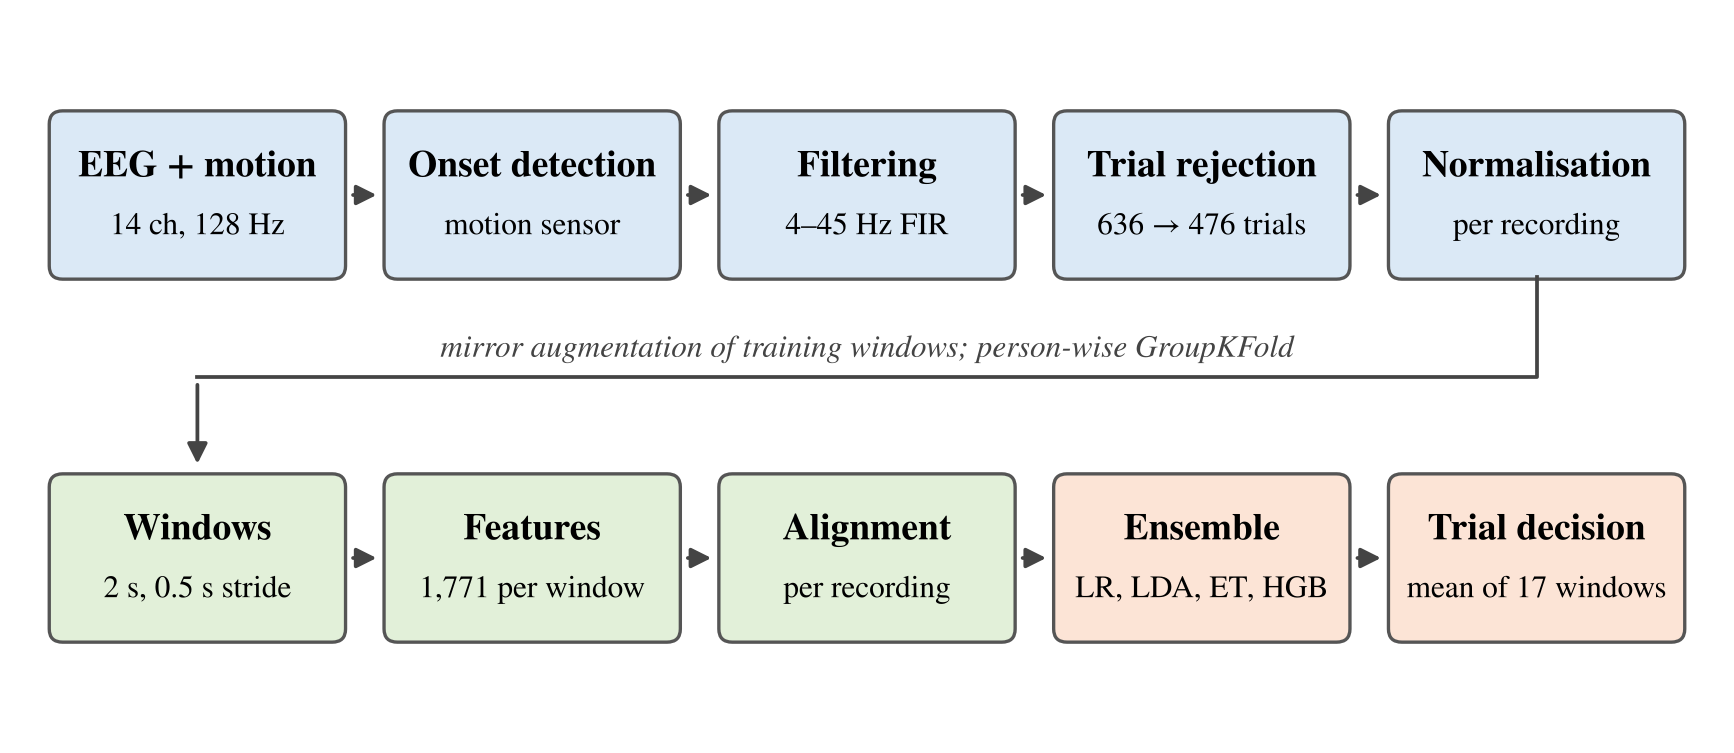
\includegraphics[width=0.72\textwidth]{figures_color/fig1_pipeline.png}
\caption{Overview of the proposed pipeline.}
\label{fig:pipeline}
\end{figure}

\subsection{Protocol and data acquisition}
Participants sat in front of a screen, kept their eyes open and followed the instructions, relaxing while a fixation cross was shown. Six movements were used: right- and left-arm flexion, right- and left-leg lifting, and right- and left-wrist rotation. Each was first performed and then imagined, giving twelve tasks in a fixed order (right arm action, right arm imagery, left arm action, and so on). As Fig.~\ref{fig:protocol}a shows, every task lasted 10~s and was followed by 5~s of rest, so the schedule spans 175~s. Some later sessions began with a resting baseline of about 50~s with eyes open and 50~s with eyes closed, which pushed the first task to roughly two minutes into the recording (Fig.~\ref{fig:protocol}b).

\begin{figure}[H]
\centering
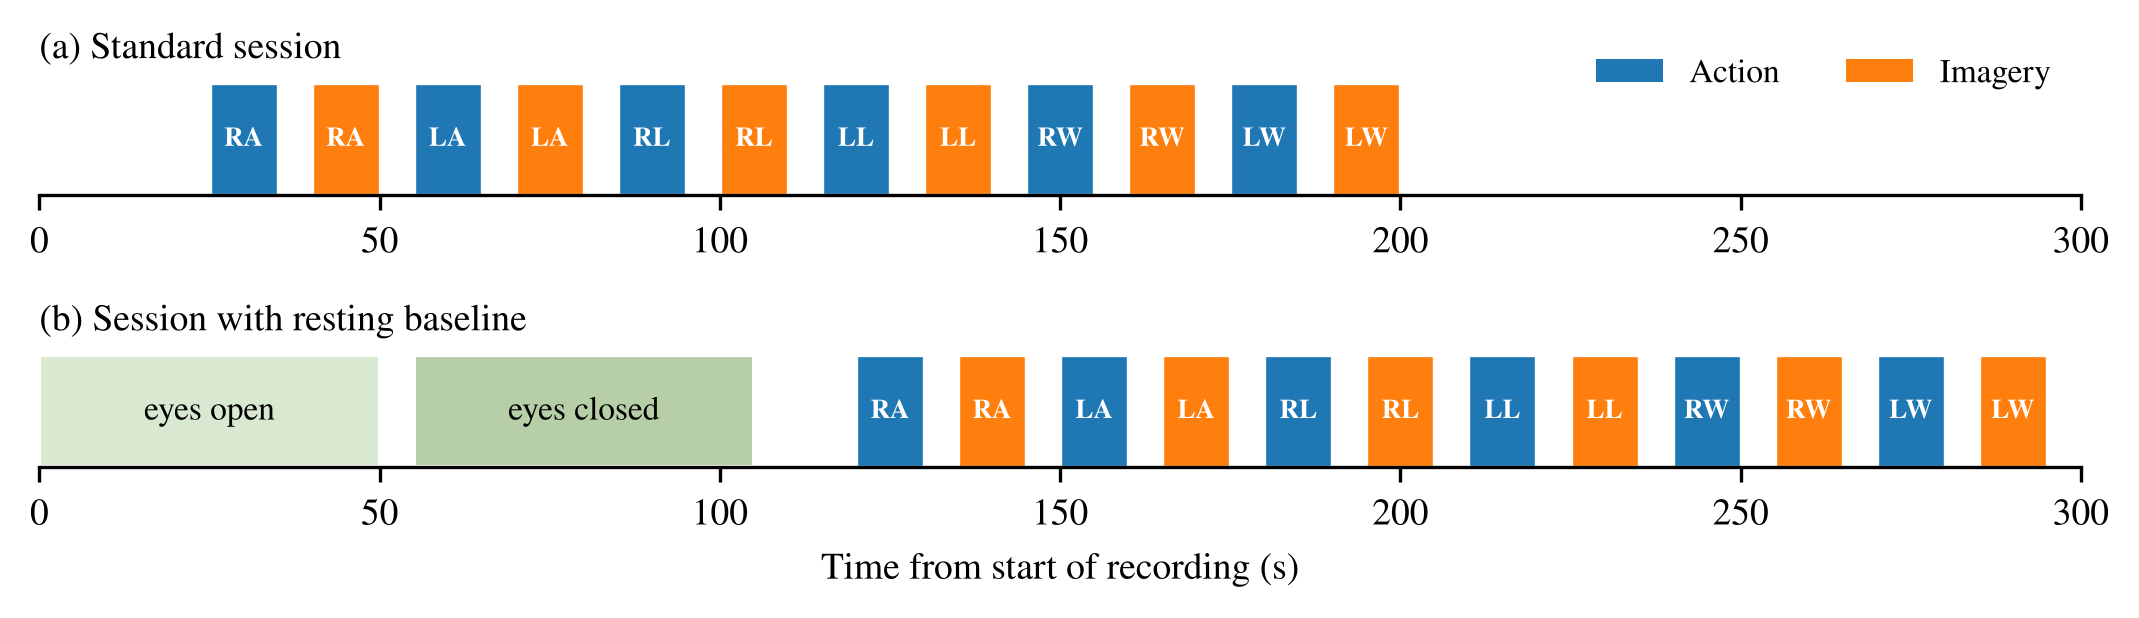
\includegraphics[width=0.9\textwidth]{figures_color/fig2_protocol.png}
\caption{Task schedule of a recording session.}
\label{fig:protocol}
\end{figure}

EEG was recorded with the Emotiv EPOC X (saline electrodes at AF3, AF4, F3, F4, F7, F8, FC5, FC6, T7, T8, P7, P8, O1 and O2; CMS/DRL reference; 128~Hz) and stored as EDF files by EmotivPRO, together with a motion file holding three accelerometer axes and four orientation components at 32~Hz. In total, 59 EEG recordings with all fourteen channels were collected from 47 participants. Each trial carries three labels: the task (12 classes), the condition, action or imagery (2 classes), and the body part (6 classes).

\subsection{Motion-guided trial onset detection}
To cut trials correctly we need to know when the first task starts. Our first pipeline assumed a fixed 15~s, but that turned out to be wrong: the delay changed from session to session and exceeded two minutes when a baseline was recorded, so most trials were cut early and labelled with the wrong task. We recovered the true onset from the motion file, using the fact that real movement shakes the head slightly while imagery does not. Motion energy was computed in 0.5~s bins as
\begin{equation}
m_b = \log \sum_{c=1}^{7} \sum_{n \in b} \left| s_c[n] - s_c[n-1] \right|,
\end{equation}
and standardised. For every candidate onset $t_0$ (0.5~s steps) the twelve-task schedule was laid over this signal, and the six action--imagery pairs were compared with a paired $t$-statistic, $t(t_0) = \bar{d}/(s_d/\sqrt{6})$, where $d_k$ is the difference in mean motion between the $k$-th action and imagery task. The onset with the largest $t$ was accepted if $t \ge 4$ and all six pairs agreed. Otherwise it was kept only if it lay within 5~s of a label-free estimate based on the recording length, since recordings normally ended about 181~s after the first task.

Fig.~\ref{fig:onset} shows one recording. Motion rises in every action block and stays low in the imagery blocks (Fig.~\ref{fig:onset}a), and the $t$-statistic peaks sharply at the detected onset of 26~s while being slightly negative at the old 15~s guess (Fig.~\ref{fig:onset}b). Across the data set, 48 recordings gave a confident onset and 5 more passed the length check; 2 were dropped because the two estimates disagreed and 4 were too short. Onsets ranged from 7.5 to 136.5~s. In the seven sessions with a confirmed eyes-closed baseline, the detected onset fell 7.3--15.5~s after the baseline ended, exactly where the schedule should begin.

\begin{figure}[H]
\centering
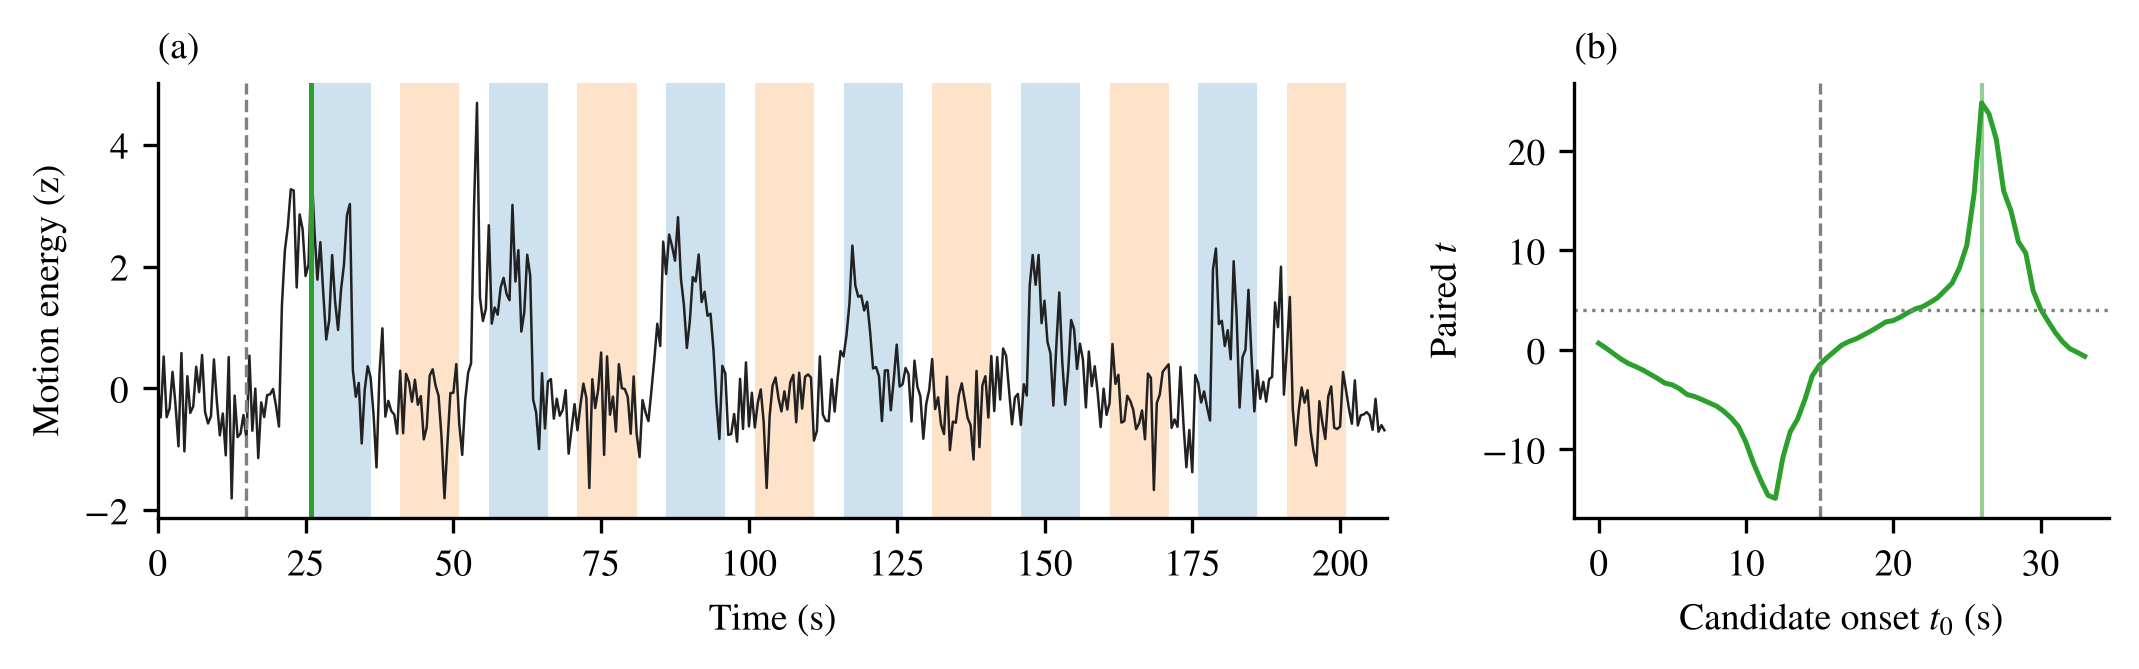
\includegraphics[width=0.85\textwidth]{figures_color/fig3_onset.png}
\caption{Motion-guided onset detection for one recording.}
\label{fig:onset}
\end{figure}

\subsection{Cleaning and normalisation}
The 53 accepted recordings were loaded with MNE-Python \citep{Gramfort2013}, reduced to the fourteen EEG channels and band-pass filtered between 4 and 45~Hz with a zero-phase FIR filter. The lower edge removes drift and most eye-blink energy; the upper edge removes muscle activity and 50~Hz mains noise, leaving the theta, mu, beta and low-gamma rhythms. Starting at the detected onset, twelve 10~s trials were cut from each recording, giving 636 trials of $14 \times 1280$ samples.

A trial was rejected if it was flat, if any sample reached 150~$\mu$V, or if its mean absolute kurtosis across channels was 10 or more. Larger values almost always come from blinks, jaw clenching or cable movement (the median trial peak was 92~$\mu$V), and high kurtosis catches sudden spikes. The amplitude rule removed 158 trials and the kurtosis rule 29, with 27 overlapping, for 160 in total (25.2\%). This left 476 clean trials from 51 recordings and 47 people: 235 action and 241 imagery trials, with 36--44 per task. Each recording was then z-scored channel by channel using the mean and standard deviation of all its retained trials; because all tasks are pooled, no labels are involved.

\subsection{Windowing and feature extraction}
Each trial was split into 2~s windows with a 0.5~s stride, giving 17 overlapping windows per trial and 8,092 in total. Every window keeps its trial index and participant identifier. Five feature families were computed from each window, 1,771 values in all:

\begin{itemize}
\item \textbf{Handcrafted (336).} For each channel: log and relative power in the theta (4--8~Hz), mu (8--12~Hz), beta (13--30~Hz) and gamma (30--45~Hz) bands from a Welch spectrum; beta/mu, mu/theta and sensorimotor ratios; variance, kurtosis, skewness and mean absolute value; Hjorth mobility and complexity \citep{Hjorth1970}; Higuchi \citep{Higuchi1988} and Petrosian fractal dimensions and the Hurst exponent; and the log energy of a three-level Daubechies-4 wavelet decomposition.
\item \textbf{Spectrogram (560).} An STFT with a 0.5~s Hann window and 50\% overlap gives 9 time frames at 2~Hz resolution. For each channel and band we keep the log power in every frame and its variance across frames.
\item \textbf{Scalogram (714).} A Morlet continuous wavelet transform at 5, 7, 10, 12, 15, 20, 25, 30, 35 and 40~Hz. For each channel we keep the log energy at every frequency in four 0.5~s segments, the ratio of 20--40~Hz to 5--15~Hz energy, and the log variance over time at each frequency.
\item \textbf{Connectivity (56).} Magnitude-squared coherence and log power asymmetry for the seven left--right electrode pairs in the four bands.
\item \textbf{Covariance (105).} A Ledoit--Wolf covariance matrix \citep{LedoitWolf2004} per window, re-centred on its recording's Riemannian mean \citep{Zanini2018} and mapped to the tangent space \citep{Barachant2012}.
\end{itemize}

The difference between the spectrogram and the scalogram is easiest to see in Fig.~\ref{fig:timefreq}, which shows the average imagery-minus-action power over all windows at four channels. Both methods show 0.8--2~dB more mu power during imagery, the expected sign of stronger desynchronisation during real movement. In the scalogram the effect is sharper in frequency and time, because the wavelet shortens its window for fast rhythms and lengthens it for slow ones, whereas the STFT uses the same 0.5~s window everywhere. Both maps also show more low-frequency power at AF3 and more high-frequency power at FC5 and T8 during action, which points to eye, head and muscle activity when people actually move.

\begin{figure}[H]
\centering
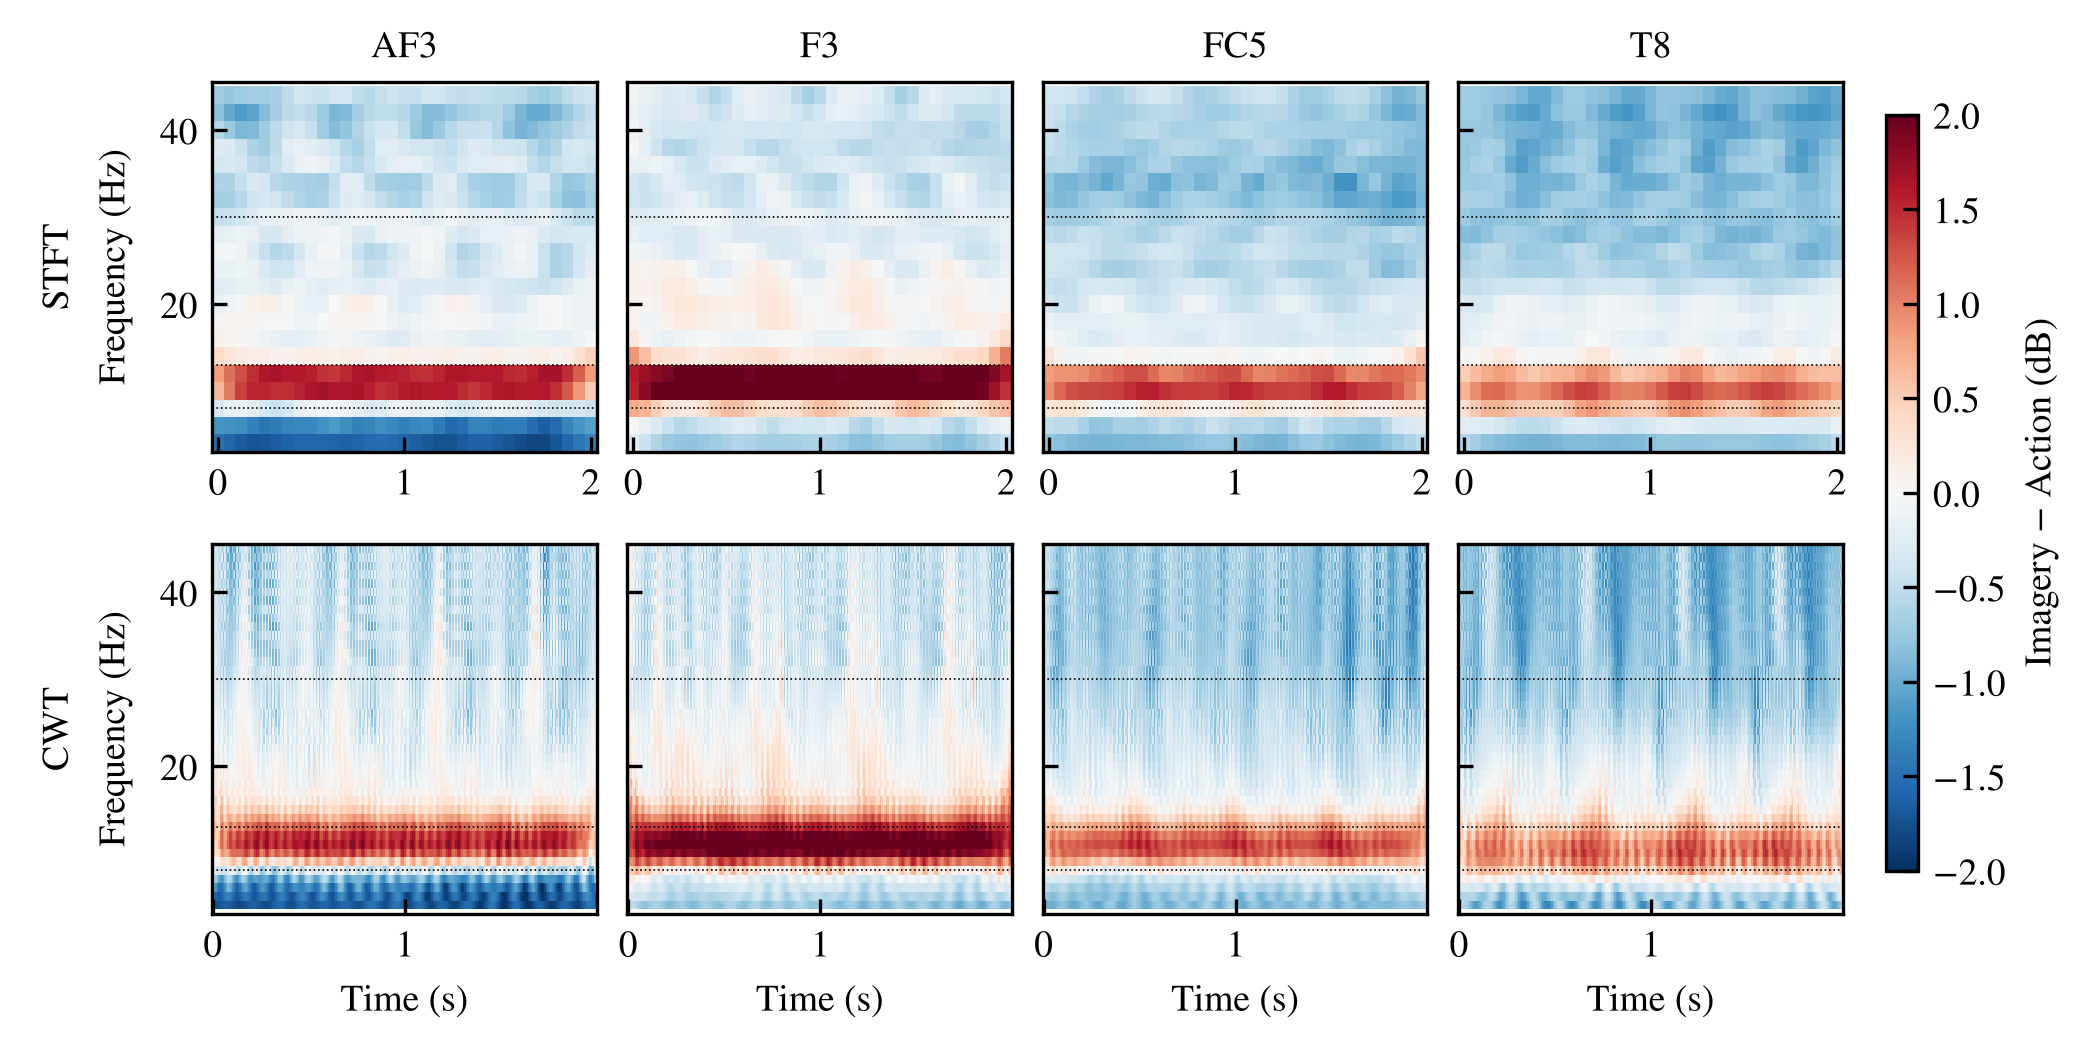
\includegraphics[width=0.78\textwidth]{figures_color/fig5_timefreq.png}
\caption{Imagery minus action power from the STFT and CWT.}
\label{fig:timefreq}
\end{figure}

\subsection{Subject-wise alignment and mirror augmentation}
Because one person's mu power can be naturally higher than another's, each of the 1,666 non-covariance features was standardised within its recording; with the covariance re-centring, this aligns all recordings without labels, so a new user needs only one unlabelled calibration session.

Because each limb is controlled mainly by the opposite hemisphere, swapping the seven left--right electrode pairs turns, roughly, a right-arm window into a left-arm one. We added such a mirrored copy of every training window (per-channel features swapped, asymmetry signs flipped, covariance permuted) with the body-side label swapped; test windows are never mirrored.

\subsection{Classifiers and evaluation}
After a scaler fitted on the training participants, four models were trained: logistic regression ($C = 0.01$), shrinkage LDA, Extra Trees (500 trees) and histogram gradient boosting (200 iterations, depth 4). Their class probabilities were averaged, and the 17 window probabilities of a trial were averaged again to give one label per trial. The same models and settings were used for every task.

As baselines we evaluated, per window and without alignment or augmentation, SVM, Random Forest, gradient boosting, Naive Bayes, AdaBoost and LDA on CSP, handcrafted and Riemannian features, plus Riemannian MDM, a hierarchical model, EEGNet \citep{Lawhern2018} and a CNN--LSTM (early stopping on 15\% of the training people).

For left-versus-right imagery, only the 241 imagery trials were used, the per-recording standardisation was computed from each recording's imagery windows only, and FBCSP with LDA \citep{Ang2012} served as the standard baseline.

All results use person-wise GroupKFold: five folds for the binary tasks and three for the six- and twelve-class tasks, so every participant is tested exactly once by a model that never saw their data. Every learned step (scaler, CSP, feature selection, tangent-space reference, classifiers and early stopping) was fitted on the training participants of each fold. We report the number of correctly classified test trials pooled over folds and the mean $\pm$ standard deviation across folds. Chance is 50\%, 16.67\% and 8.33\% for two, six and twelve classes.

%% ===================================================================
\section{Results and Discussion}\label{sec:results}

\subsection{Main results}
Table~\ref{tab:main} gives the accuracy of the proposed system. Four out of five action-versus-imagery trials of unseen people were classified correctly, about 30 points above chance, while body part and the exact task reached 1.6 and 2.6 times chance. Averaging the 17 windows of a trial added 11.7 points for action versus imagery and 5.7 points for the two multi-class tasks over single-window decisions. Fold accuracy for action versus imagery ranged from 71.3\% to 89.7\%, so decoding depends strongly on the individual.

\begin{table}[!htbp]
\centering
\caption{Accuracy of the proposed system (person-wise GroupKFold).}
\label{tab:main}
\footnotesize
\begin{tabular}{@{}lcccc@{}}
\toprule
Task & Chance & Trials (pooled) & Trials (fold mean) & Windows (fold mean) \\
\midrule
Action vs.\ imagery & 50.00 & \textbf{80.25} (382/476) & 80.19 $\pm$ 6.59 & 68.53 $\pm$ 3.59 \\
Body part (6) & 16.67 & \textbf{26.68} (127/476) & 26.68 $\pm$ 1.79 & 21.01 $\pm$ 0.42 \\
Twelve tasks & 8.33 & \textbf{21.43} (102/476) & 21.42 $\pm$ 1.21 & 15.75 $\pm$ 0.83 \\
Left vs.\ right imagery & 50.00 & \textbf{58.09} (140/241) & 58.10 $\pm$ 5.91 & 52.65 $\pm$ 2.74 \\
\botrule
\end{tabular}
\end{table}

\subsection{What each component adds}
Table~\ref{tab:ablation} separates the contributions. No single classifier won every task, while the ensemble stayed within about a point of the best one. Subject-wise alignment mattered most. Without it, action-versus-imagery accuracy fell from 79.62\% to 70.17\% (379 vs.\ 334 trials), so much of the difference between people behaves like a simple offset in feature values. Mirror augmentation then added 3, 5 and 5 correct trials on the three tasks. These gains are small, but consistent, and they halved the fold-to-fold variation of the multi-class tasks.

\begin{table}[!htbp]
\centering
\caption{Trial-level accuracy (fold mean $\pm$ SD, \%) of the components.}
\label{tab:ablation}
\footnotesize
\begin{tabular}{@{}lccc@{}}
\toprule
Model & Action/imagery & Body part & Twelve tasks \\
\midrule
Logistic regression & 79.96 $\pm$ 7.71 & 23.51 $\pm$ 1.69 & 17.67 $\pm$ 2.86 \\
LDA & 76.19 $\pm$ 7.94 & 23.50 $\pm$ 3.13 & 19.55 $\pm$ 2.40 \\
Extra Trees & 77.88 $\pm$ 6.81 & 22.49 $\pm$ 1.01 & 18.92 $\pm$ 1.44 \\
HistGB & 78.74 $\pm$ 5.01 & 26.48 $\pm$ 2.91 & 19.96 $\pm$ 0.86 \\
Ensemble, no alignment & 70.14 $\pm$ 5.51 & 23.77 $\pm$ 2.36 & 19.34 $\pm$ 1.74 \\
Ensemble, no augmentation & 79.56 $\pm$ 6.37 & 25.60 $\pm$ 3.59 & 20.41 $\pm$ 5.59 \\
\textbf{Ensemble + augmentation} & \textbf{80.19 $\pm$ 6.59} & \textbf{26.68 $\pm$ 1.79} & \textbf{21.42 $\pm$ 1.21} \\
\botrule
\end{tabular}
\end{table}

\subsection{Comparison with other methods}
Table~\ref{tab:baselines} compares the system with the baselines. Even at window level it was best on every task. The strongest conventional pipelines reached 62--64\% for action versus imagery and 20--21\% for body part, with Riemannian features consistently competitive. EEGNet matched the classical baselines for action versus imagery (62.15\%) but stayed near chance for body part and the exact task, and the CNN--LSTM was weaker; with fewer than 40 training people per fold, the networks probably could not learn features that transfer to new people \citep{Roy2019}.

\begin{table}[!htbp]
\centering
\caption{Comparison methods (window level, fold mean $\pm$ SD, \%).}
\label{tab:baselines}
\footnotesize
\begin{tabular}{@{}lccc@{}}
\toprule
Model & Action/imagery & Body part & Twelve tasks \\
\midrule
All features + HistGB & 64.45 $\pm$ 2.35 & 19.71 $\pm$ 0.13 & 12.90 $\pm$ 0.03 \\
CSP + all + Riemann + SVM & 62.89 $\pm$ 3.73 & 20.62 $\pm$ 0.59 & 14.32 $\pm$ 1.27 \\
Riemannian + SVM & -- & 20.70 $\pm$ 1.13 & 13.17 $\pm$ 1.78 \\
Riemannian MDM & 62.31 $\pm$ 4.64 & 19.92 $\pm$ 1.44 & 12.05 $\pm$ 1.37 \\
Hierarchical & -- & -- & 13.83 \\
EEGNet & 62.15 $\pm$ 3.70 & 17.49 $\pm$ 1.23 & 10.61 $\pm$ 1.31 \\
CNN--LSTM & 58.38 $\pm$ 4.87 & -- & -- \\
\textbf{Proposed (window)} & \textbf{68.53 $\pm$ 3.59} & \textbf{21.01 $\pm$ 0.42} & \textbf{15.75 $\pm$ 0.83} \\
\textbf{Proposed (trial)} & \textbf{80.19 $\pm$ 6.59} & \textbf{26.68 $\pm$ 1.79} & \textbf{21.42 $\pm$ 1.21} \\
\botrule
\end{tabular}
\end{table}

\subsection{Spectrogram versus scalogram}
To measure each representation on its own, we re-ran the pipeline (without augmentation) with one feature family at a time. Fig.~\ref{fig:families} shows that the scalogram beat the spectrogram on all three tasks: by 1.05 points for action versus imagery (77.52\% vs.\ 76.47\%), 3.78 points for body part (21.85\% vs.\ 18.07\%) and 4.62 points for the exact task (19.54\% vs.\ 14.92\%). With the spectrogram alone, body part was barely above chance. As Fig.~\ref{fig:timefreq} suggests, the 2~Hz resolution of the fixed STFT window blurs the mu and beta bands, which the wavelet keeps apart. On its own, the scalogram equalled the 336 handcrafted features for action versus imagery and the exact task, and combining STFT and CWT gave the best twelve-task score in this comparison (20.80\%). For body part, adding handcrafted, connectivity and covariance features raised accuracy from about 21\% to 25.63\%, so locating the limb also needs spatial information.

\begin{figure}[H]
\centering
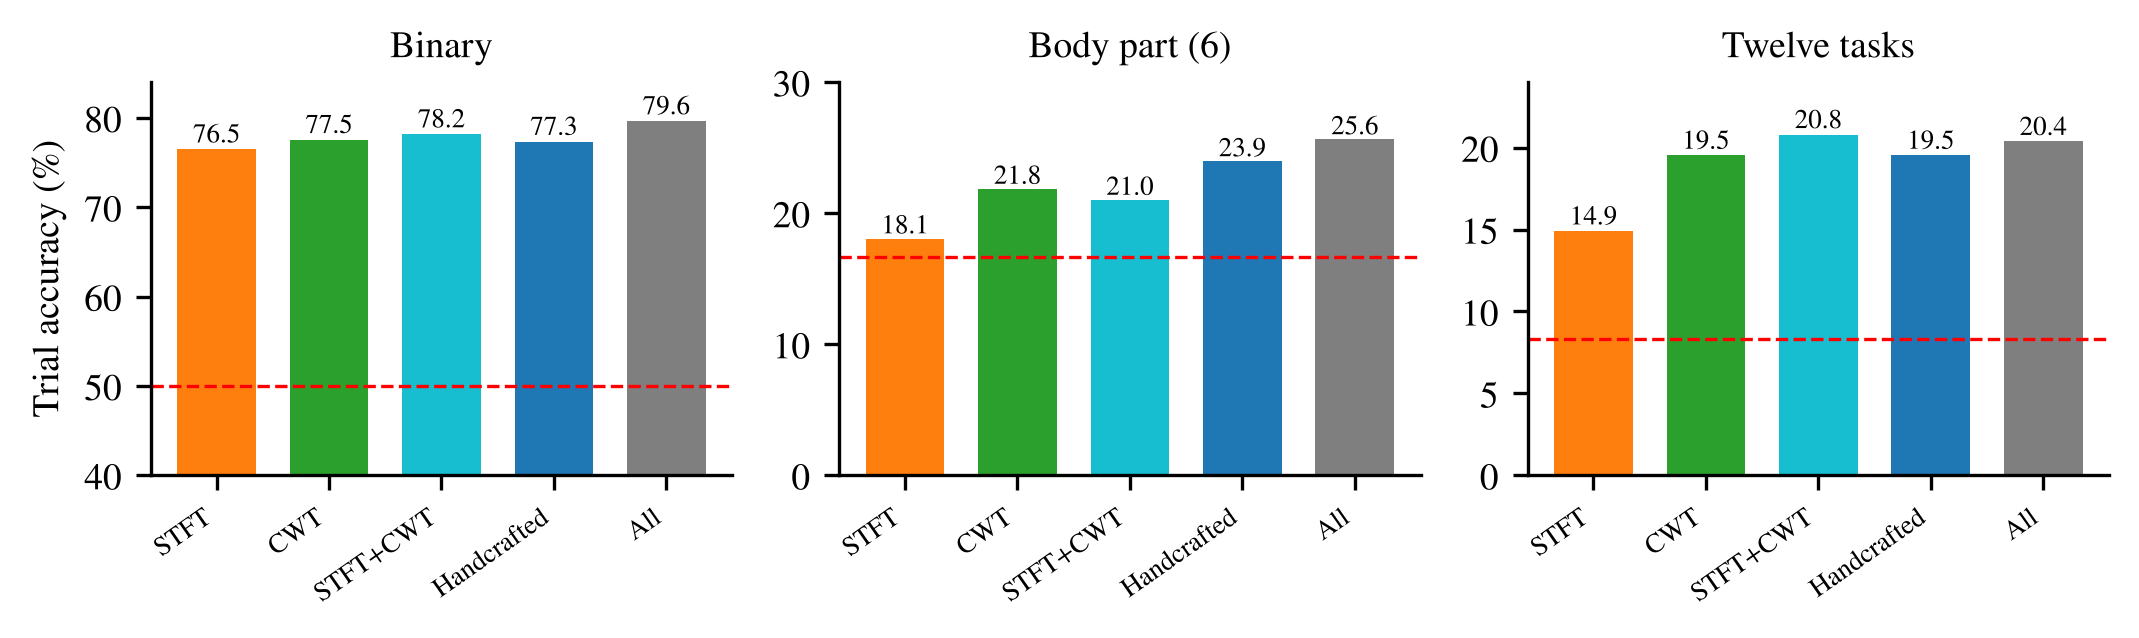
\includegraphics[width=0.9\textwidth]{figures_color/fig6_families.png}
\caption{Accuracy with single feature families.}
\label{fig:families}
\end{figure}

\subsection{Informative features and errors}
Fig.~\ref{fig:importance} ranks the features for action versus imagery by their ANOVA $F$-score, computed on the training people of each fold. Almost all of the top features are mu-band measures (relative mu power, the mu/theta ratio and the sensorimotor ratio), in line with the desynchronisation seen in Fig.~\ref{fig:timefreq}, and three scalogram features also reach the top 20. The strongest features come from the frontal channels AF3, AF4, F3 and F4, though, rather than from the motor cortex, which the headset does not cover. These sites also pick up eye and muscle activity, so part of the action-versus-imagery accuracy probably reflects the side effects of moving.

\begin{figure}[H]
\centering
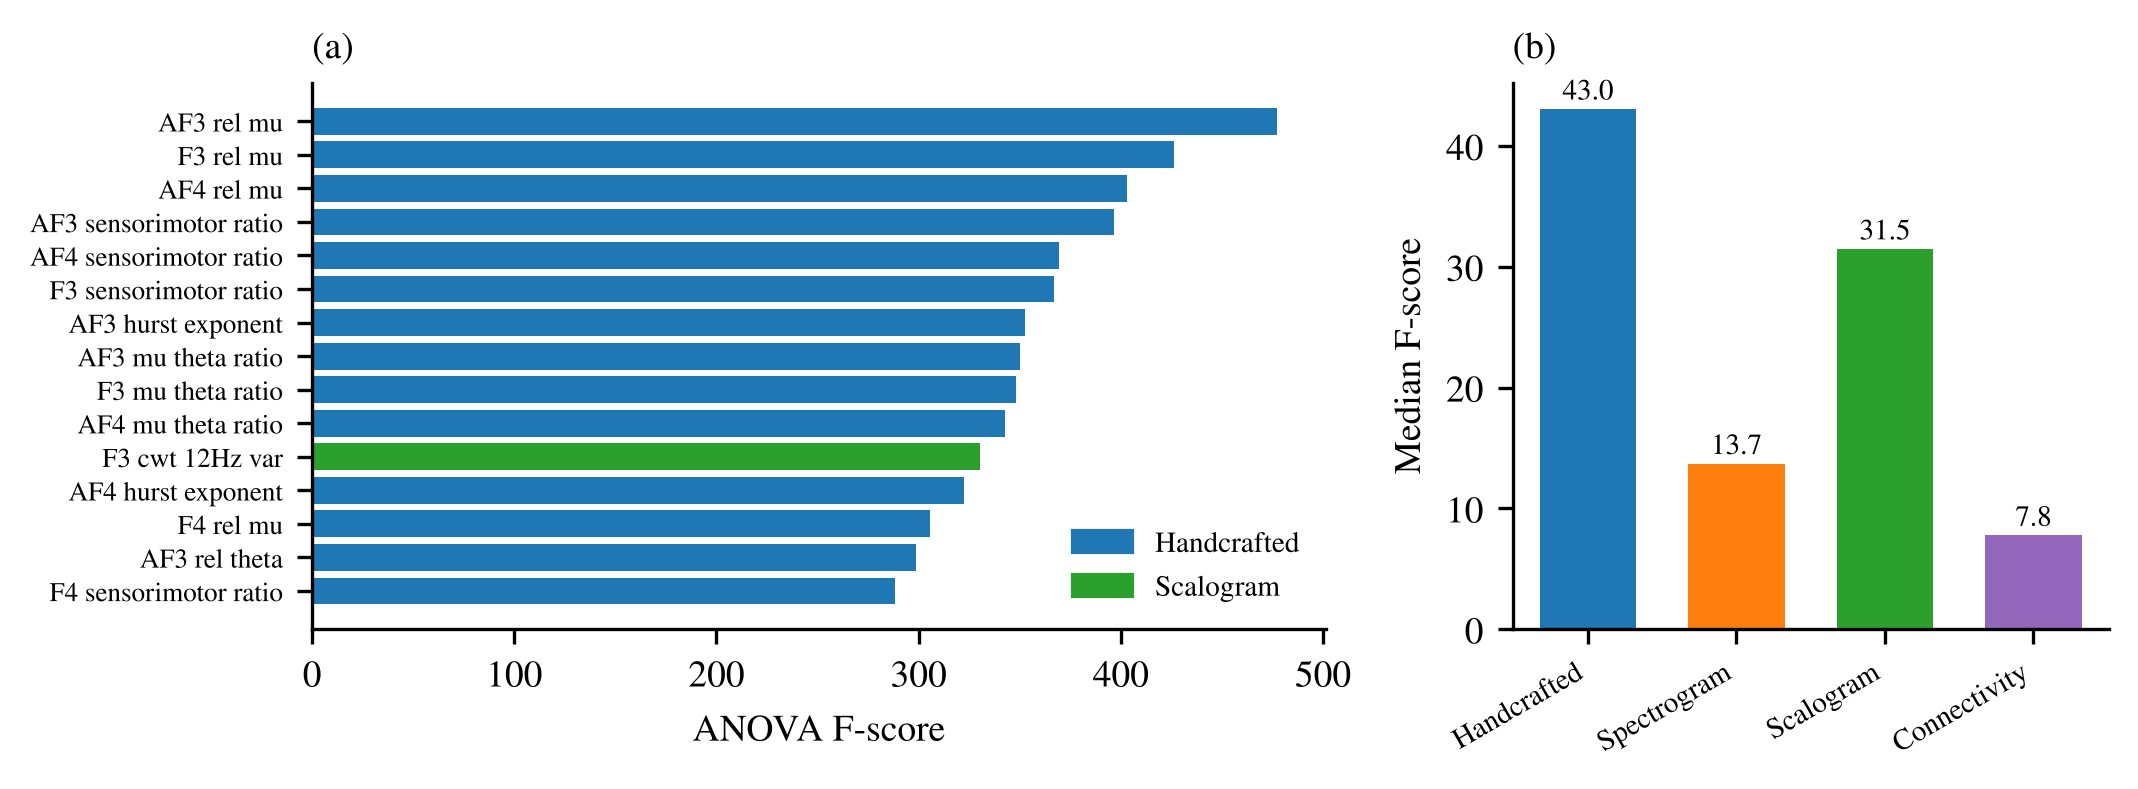
\includegraphics[width=0.78\textwidth]{figures_color/fig8_importance.png}
\caption{Feature importance for action versus imagery.}
\label{fig:importance}
\end{figure}

The confusion matrices in Fig.~\ref{fig:confusion} show where the errors lie. For action versus imagery they are balanced (77.0\% of action and 83.4\% of imagery trials correct). For body part, the classifier recognised the limb type (arm, leg or wrist) in 46.0\% of trials against 33.3\% by chance, but the side in only 54.6\%; right arm (37.8\%) and right wrist (31.0\%) were recognised best, and left wrist worst (13.5\%). In the twelve-task problem, the action/imagery part of the label was right in 78.2\% of trials but the body part in only 25.8\%. Most errors therefore come from telling limbs and sides apart, which is expected without electrodes over C3 and C4.

\begin{figure}[H]
\centering
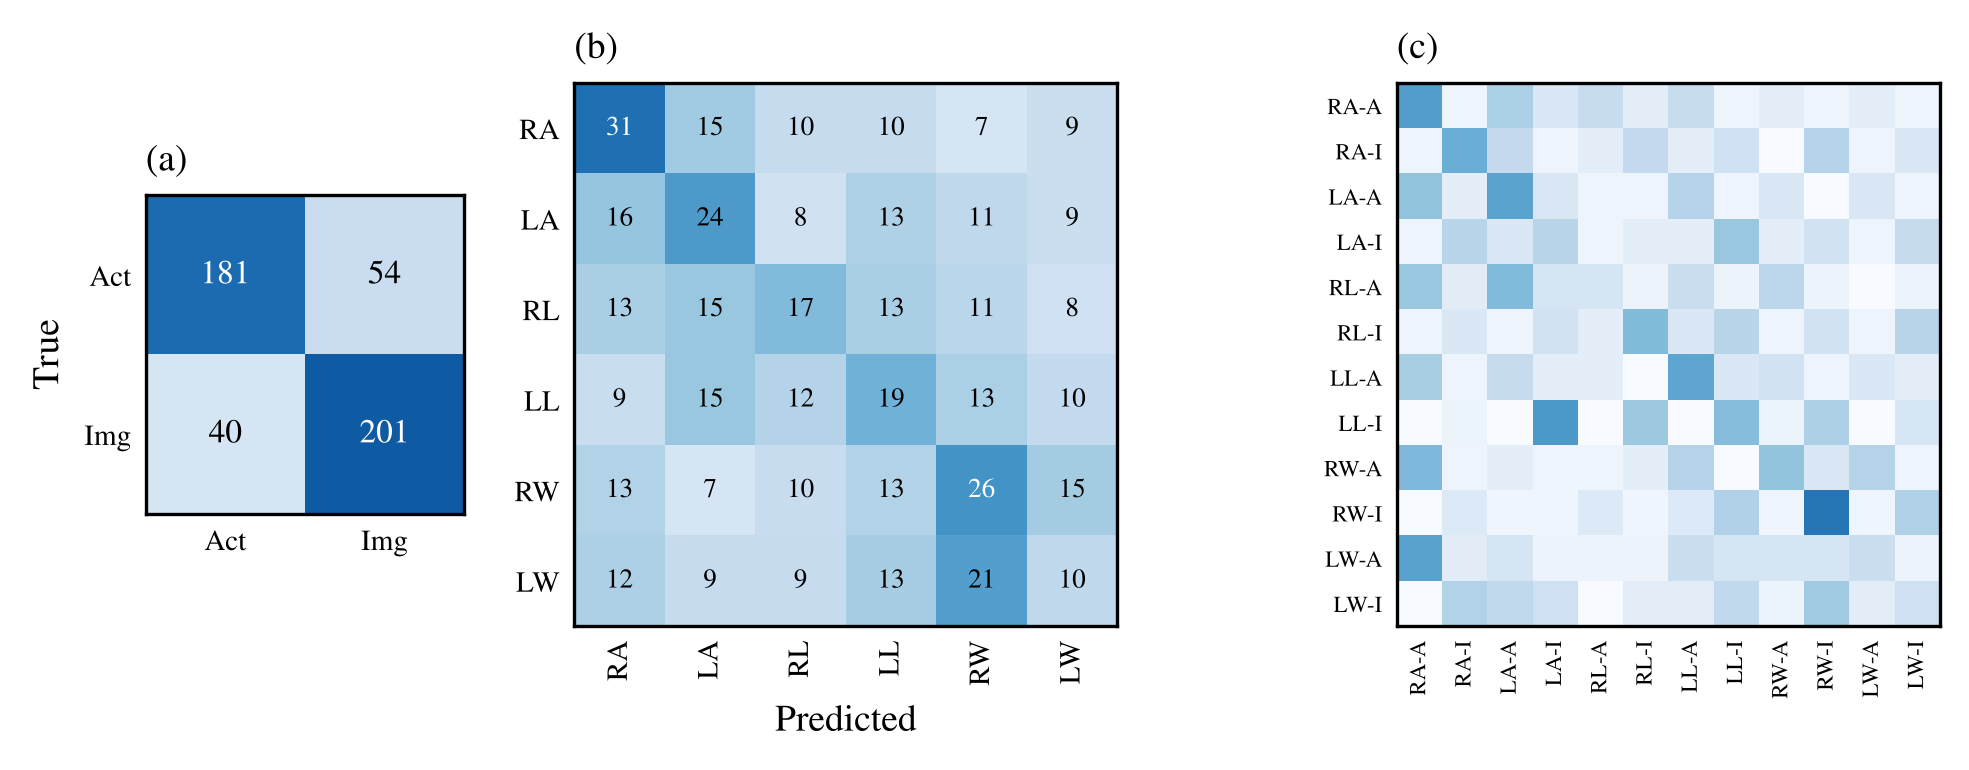
\includegraphics[width=0.82\textwidth]{figures_color/fig7_confusion.png}
\caption{Trial-level confusion matrices pooled over test folds.}
\label{fig:confusion}
\end{figure}

\subsection{Left versus right imagery}
Table~\ref{tab:lr} shows that the side of an imagined movement was hard to decode across people. The standard FBCSP + LDA approach stayed at chance (52.70\%), as did the ensemble with the usual calibration (53.53\%). Calibrating each person on their imagery trials alone, together with mirror augmentation, lifted accuracy to 58.09\% ($p = 0.007$, one-sided binomial test). Arm imagery was by far the most separable (74.07\%), probably because the arm area lies close to the FC5/FC6 electrodes, while leg and wrist did not reach significance. Two cautions apply. The right-side task always came 30~s before the left-side one, so slow drift during a session could help separate them, especially for the arm pair at the start. And this configuration was the best of six we tried, although $p$ stays below 0.05 (0.043) after a Bonferroni correction. A recording with randomised task order is needed to confirm the result.

\begin{table}[!htbp]
\centering
\caption{Left versus right motor imagery (trial level).}
\label{tab:lr}
\footnotesize
\begin{tabular}{@{}lccc@{}}
\toprule
Method & Correct & Accuracy (\%) & $p$ \\
\midrule
FBCSP + LDA & 127/241 & 52.70 & 0.22 \\
Ensemble, standard calibration & 129/241 & 53.53 & 0.15 \\
\textbf{Ensemble, imagery-only calibration} & \textbf{140/241} & \textbf{58.09} & \textbf{0.007} \\
\quad arm / leg / wrist & 60/81, 46/78, 48/82 & 74.07, 58.97, 58.54 & $<$0.001, 0.07, 0.08 \\
\botrule
\end{tabular}
\end{table}

\subsection{Validity of the evaluation}
An earlier version of this work reported more than 94\% accuracy because random window-level splits let overlapping windows of the same person, and feature selection fitted on all data, leak into testing. We therefore ran three checks on the final pipeline. First, no participant, recording or trial ever appeared on both sides of a split, and no recording occurred twice in the data set. Second, we shuffled the labels within each recording and ran the whole pipeline again three times; accuracy fell to chance (49.37\%, 54.62\% and 48.32\% for action versus imagery; 18.70\%, 17.65\% and 18.49\% for body part), as it should. Third, because each onset was chosen from the action--imagery motion contrast, we shifted all onsets by $\pm$2~s. Body-part accuracy hardly changed, but action-versus-imagery accuracy dropped by about 3 points (79.20\% to 76.16\% and 75.85\% with the fast feature families), so that result may be optimistic by up to 3 points. It stays above 75\% in every case.

\subsection{Limitations}
The EPOC X lacks electrodes over the central motor strip, which limits body-part and left/right decoding. The data set holds about 40 trials per task, trial rejection removed a quarter of them, and ICA could recover more data while separating cortical from eye and muscle activity. The fixed task order may confound slow drift with the labels, the method choices were made on the same participants without an untouched test group, and all results are offline.

%% ===================================================================
\section{Conclusion}\label{sec:conclusion}

This study presented a subject-independent pipeline for classifying motor action and motor imagery from a 14-channel Emotiv EPOC X. Recovering trial onsets from the motion sensor, standardising features per recording and deciding per trial made the main difference. With an ensemble of four classifiers trained with hemispheric mirror augmentation, the system reached 80.25\% for action versus imagery, 26.68\% for six body parts, 21.43\% for twelve tasks and 58.09\% for left versus right imagery on people it had never seen. A label-permutation test confirmed that these results are not caused by leakage, and the system outperformed CSP, Riemannian and deep-learning baselines under the same conditions. The Morlet scalogram was consistently more informative than the STFT spectrogram. Without central electrodes, identifying the limb and side remains far harder than telling movement from imagery. Future work will use randomised task order, more imagery repetitions, ICA-based artefact removal and online testing.

\section{Data availability}
Data will be available upon request.

\section{Author Contributions}
All authors read and approved the final manuscript.

\section{Funding}
All necessary funding, including support for open access publication, is provided by Amrita Vishwa Vidyapeetham, India.

\bibliography{bibliography}

\end{document}
